\documentclass[letterpaper, 12pt]{report}

\usepackage[utf8]{inputenc}
\usepackage[english, spanish]{babel}

\usepackage{fullpage}
\usepackage{graphicx}
\usepackage{amsmath}
\usepackage{enumitem}
\usepackage{chngcntr}
\usepackage{setspace}
\usepackage{xurl}
\usepackage{csquotes}
\usepackage{float}
\usepackage{verbatim}
\usepackage{tabularx}
\usepackage{amsmath}
\usepackage{caption}
\usepackage{bm}
\usepackage{wrapfig}
\usepackage{siunitx}
\usepackage{multirow}

\counterwithin{figure}{section}
\renewcommand{\thefigure}{\arabic{figure}}
\renewcommand{\thesection}{\arabic{section}}
\renewcommand{\thesubsection}{\thesection.\arabic{subsection}}
\renewcommand{\baselinestretch}{2}
\renewcommand{\thefigure}{\arabic{figure}}

\usepackage[style=apa, maxnames=6, minnames=3]{biblatex}
\DefineBibliographyStrings{english}{%chktex-file 1 chktex-file 6
      andothers = {\em et\addabbrvspace al\adddot}
}

\addbibresource{./Bibliography/bibliography.bib}

\DeclareCiteCommand{\textcite}
{\usebibmacro{prenote}}
{\usebibmacro{citeindex}%
      \printnames{labelname}%
      \setunit{\addcomma\addspace}%
      \printfield{year}%
      \setunit{\addcomma\addspace}%
      \printfield{title}}
{\multicitedelim}
{\usebibmacro{postnote}}

\DeclareCiteCommand{\cite}
{\usebibmacro{prenote}}
{\usebibmacro{citeindex}%
      (\printnames{labelname}%
      \setunit{\addcomma\addspace}%
      \printfield{year}%
      \setunit{\addcomma\addspace}%
      \printfield{title})}
{\multicitedelim}
{\usebibmacro{postnote}}

\usepackage{array}
\usepackage{enumitem}

\setlength{\parskip}{\baselineskip}

\newcommand{\bolditalic}[1]{\textbf{\textit{#1}}}

\renewcommand{\comment}[1]{{\small $\ll$#1$\gg$}}

% chktex-file 24
% chktex-file 44

\begin{document}

\begin{titlepage}
	\centering
	
\includegraphics[width=0.3\textwidth]{Images/logo_utb.png}\par\vspace{1cm}
	{\scshape\LARGE Universidad Tecnológica de Bolívar \par}
	\vspace{.5cm}

	{\scshape\Large BASE DE DATOS \par}
	\vspace{.7cm}

	\slshape {\Large \bfseries{}Taller no. 1\\}
	\slshape {\small \bfseries{}Modelo E-R}
	\vspace{.6cm}

	\slshape {\itshape{} Mauro González, T00067622 \\}
	\slshape {\itshape{} María Valentina Serna González, T00067756 \\}
	\slshape {\itshape{} Jorge Andrés Herrera Monsalve, T00068111 \\}
	\slshape {\itshape{} Juan Jose Jimenez Guardo, T00068278 \\}
	\slshape {\itshape{} Aarón Dalí López Fortich, T00068394 \\}
	\vfill
	Revisado Por \\
	Maria Fernanda Medina Reyes\\
	{\large \today\par}
\end{titlepage}

\section{Review Questions}

Define the following terms:

\begin{itemize}[label=$\triangleright$]
	\item \textbf{Entity}: En la informática, una entidad puede ser un objeto
	      o un concepto en el espacio, el cual se representa en un sistema
	      de información. En bases de datos, una entidad puede ser un lugar,
	      un objeto, una persona o un concepto. En la programación orientada a
	      objetos, una identidad puede ser una clase que representa a un usuario
	      con propiedades tales como, correo, edad, nombre y métodos que se
	      usarían para interactuar con esos datos.

	      \nocite{Unir_2023}

	\item \textbf{Attribute}: Se refiere a una característica o
	      propiedad de un objeto, clase o entidad que lo puede describir
	      y definir. Existen características importantes de los atributos.

	      \nocite{Unir_2023}

	      \begin{itemize}
		      \item Los atributos describen las propiedades de un objetos,
		            entidad o clase; por ejemplo, la clase “persona”, los
		            atributos de esta clase serian nombre, edad, genero, altura, etc.

		      \item Los atributos son utilizados para mantener el
		            estado de los objetos, es decir, si estamos creando un objeto
		            que pueda representar una cuenta de banco, los atributos
		            incluyen, fecha de apertura de la cuenta de banco,
		            saldo, titular etc.

		      \item Los atributos manejan diferentes tipos de accesos,
		            los cuales permiten leer y modificar su valor. Esto ayuda
		            a garantizar la seguridad de los datos.

		      \item Los atributos, pueden tener diferentes tipos de datos,
		            como números enteros, booleanos, decimales, cadenas
		            de texto etc.
	      \end{itemize}


	\item \textbf{Attribute value}: En la informática se refiere
	      al valor asociado a un atributo en un contexto especifico; es
	      simplemente un valor especifico que un atributo tiene en un
	      momento dado para un objeto, entidad o clase en particular.

	      \nocite{UNIVERSIDAD_DON_BOSCO}

	\item \textbf{Relationship}: Hace referencia a la relación
	      que existe entre dos o mas entidades, componentes, objetos o
	      elementos que se encuentran dentro de un sistema o un conjunto
	      de datos. Específicamente en el diseño de bases de satos, las
	      relaciones definen como se conectan las tablas entre sí,
	      mediante claves primarias y foráneas. Ejemplo, una tabla
	      de “Cliente” tiene una relación de “ordenes” a través de
	      una clave foránea que une los clientes con las ordenes que han realizado.

	\item \textbf{Composite attribute}: Es un atributo que se puede
	      componer de múltiples partes que están relacionados entre sí, y
	      que se manejan como una sola unidad de información dentro de una
	      entidad en la base de datos.

	\item \textbf{Multivalued attribute}: Es un termino que se usa
	      en bases de datos para describir que es un atributo que puede
	      tener múltiples valores para una sola instancia de una entidad
	      en la base de datos, y esto permite que pueda representar
	      información mas compleja y detallada sobre las entidades.

	\item \textbf{Derived attribute}: Es un atributo derivado es un
	      atributo cuyo valor se calcula o se deriva dinámicamente a partir de otros
	      atributos almacenados en la base de datos, lo que ayuda a mantener la
	      integridad de los datos y evitar la redundancia de información, por
	      ejemplo si se considera la entidad “Persona” con atributos como: fecha
	      de nacimiento y edad. L edad es un atributo derivado, debido a que su
	      valor se puede calcular en función de la fecha de nacimiento.

	\item \textbf{Complex attribute}: un atributo complejo es un tipo de
	      atributo en una base de datos que está compuesto por sub-atributos o
	      componentes internos que tienen estructuras de datos más elaboradas
	      que simples valores, lo que permite representar información detallada
	      y estructurada dentro de una entidad; Por ejemplo, considera una
	      entidad ``Persona'' con un atributo complejo llamado ``Dirección'',
	      donde la dirección se compone de varios sub-atributos como calle,
	      ciudad, estado y código postal.

	\item \textbf{Key attribute}: son fundamentales para establecer
	      relaciones entre las tablas de una base de datos y para garantizar
	      la integridad de los datos. Permiten la identificación única de cada
	      registro y facilitan las operaciones de búsqueda y recuperación de
	      datos en la base de datos.

	\item \textbf{Value set} (domain): Es un medio para definir y
	      aplicar restricciones sobre los valores que pueden almacenarse
	      en una columna específica de una tabla en una base de datos. Esto
	      contribuye a mantener la integridad y consistencia de los datos
	      almacenados.
\end{itemize}

\section{Notation for ER diagrams}

\textit{Complete the notations using: Chen Notation \@{} Entity / Relationship}

\begin{table}[H]
	\begin{center}
		\begin{tabularx}{.8\linewidth}{|>{\centering\arraybackslash}X|>{\centering\arraybackslash}X|}
			\hline
			\textbf{Meaning} & \textbf{Symbol} \\\hline
		\end{tabularx}
	\end{center}
\end{table}

\vspace{-1.2cm}

\begin{table}[H]
	\begin{center}
		\begin{tabularx}{.8\linewidth}{|>{\centering\arraybackslash}X|>{\centering\arraybackslash}X|}
			\hline
			\multirow{4}{*}{Entity} & \begin{center} 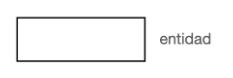
\includegraphics[width=.9\linewidth]{./Images/Entidad.png}  \end{center} \\\hline
		\end{tabularx}
	\end{center}
\end{table}

\vspace{-1.2cm}

\begin{table}[H]
	\begin{center}
		\begin{tabularx}{.8\linewidth}{|>{\centering\arraybackslash}X|>{\centering\arraybackslash}X|}
			\hline
			\multirow{3}{*}{Weak Entity} & \begin{center} 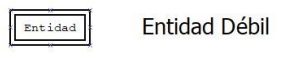
\includegraphics[width=.9\linewidth]{./Images/EntidadDebil.png}  \end{center} \\\hline
		\end{tabularx}
	\end{center}
\end{table}

\vspace{-1.2cm}

\begin{table}[H]
	\begin{center}
		\begin{tabularx}{.8\linewidth}{|>{\centering\arraybackslash}X|>{\centering\arraybackslash}X|}
			\hline
			\multirow{4}{*}{Relationship} & \begin{center} 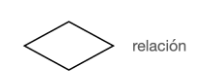
\includegraphics[width=.9\linewidth]{./Images/Relacion.png}  \end{center} \\\hline
		\end{tabularx}
	\end{center}
\end{table}

\vspace{-1.2cm}

\begin{table}[H]
	\begin{center}
		\begin{tabularx}{.8\linewidth}{|>{\centering\arraybackslash}X|>{\centering\arraybackslash}X|}
			\hline
			\multirow{4}{*}{Attribute} & \begin{center} 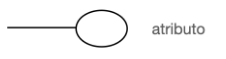
\includegraphics[width=.9\linewidth]{./Images/Atributo.png}  \end{center} \\\hline
		\end{tabularx}
	\end{center}
\end{table}

\vspace{-1.2cm}

\begin{table}[H]
	\begin{center}
		\begin{tabularx}{.8\linewidth}{|>{\centering\arraybackslash}X|>{\centering\arraybackslash}X|}
			\hline
			\multirow{3}{*}{Key Attribute} & \begin{center} 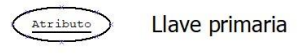
\includegraphics[width=.9\linewidth]{./Images/LlavePrimaria.png}  \end{center} \\\hline
		\end{tabularx}
	\end{center}
\end{table}

\vspace{-1.2cm}

\begin{table}[H]
	\begin{center}
		\begin{tabularx}{.8\linewidth}{|>{\centering\arraybackslash}X|>{\centering\arraybackslash}X|}
			\hline
			\multirow{5}{*}{Multivalued Attribute} & \begin{center} 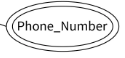
\includegraphics[width=.9\linewidth]{./Images/MultiEvaluado.png}  \end{center} \\\hline
		\end{tabularx}
	\end{center}
\end{table}

\vspace{-1.2cm}

\begin{table}[H]
	\begin{center}
		\begin{tabularx}{.8\linewidth}{|>{\centering\arraybackslash}X|>{\centering\arraybackslash}X|}
			\hline
			\multirow{6}{*}{Composite Attribute} & \begin{center} 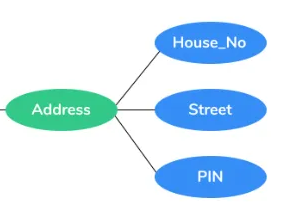
\includegraphics[width=.9\linewidth]{./Images/Compuesto.png}  \end{center} \\\hline
		\end{tabularx}
	\end{center}
\end{table}

\vspace{-1.2cm}

\begin{table}[H]
	\begin{center}
		\begin{tabularx}{.8\linewidth}{|>{\centering\arraybackslash}X|>{\centering\arraybackslash}X|}
			\hline
			\multirow{6}{*}{Derived Attribute} & \begin{center} 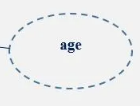
\includegraphics[width=.9\linewidth]{./Images/Derivado.png}  \end{center} \\\hline
		\end{tabularx}
	\end{center}
\end{table}

\vspace{-1.2cm}

\begin{table}[H]
	\begin{center}
		\begin{tabularx}{.8\linewidth}{|>{\centering\arraybackslash}X|>{\centering\arraybackslash}X|}
			\hline
			\multirow{4}{*}{Total Participation of E2 in R} & \begin{center} 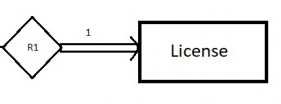
\includegraphics[width=.9\linewidth]{./Images/ParticipacionTotal.png}  \end{center} \\\hline
		\end{tabularx}
	\end{center}
\end{table}

\vspace{-1.2cm}

\begin{table}[H]
	\begin{center}
		\begin{tabularx}{.8\linewidth}{|>{\centering\arraybackslash}X|>{\centering\arraybackslash}X|}
			\hline
			\multirow{4}{*}{Cardinality Ratio 1:N} & \begin{center} 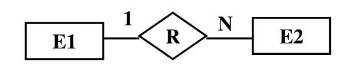
\includegraphics[width=.9\linewidth]{./Images/Cardinalidad.png}  \end{center} \\\hline
		\end{tabularx}
	\end{center}
\end{table}

\vspace{-1.2cm}

\begin{table}[H]
	\begin{center}
		\begin{tabularx}{.8\linewidth}{|>{\centering\arraybackslash}X|>{\centering\arraybackslash}X|}
			\hline
			\multirow{3}{*}{\begin{tabular}{@{}c@{}}Structural Constraint (min, max)\\ R E on Participation of E in R\end{tabular}} & \begin{center} 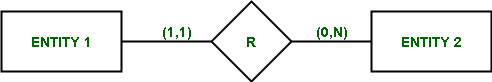
\includegraphics[width=.9\linewidth]{./Images/Constraints.png}  \end{center} \\\hline
		\end{tabularx}
	\end{center}
\end{table}

\section{Diagrama E\@{}-\@{}R:\@{} Pedidos}

\begin{figure}[H]
	\begin{center}
		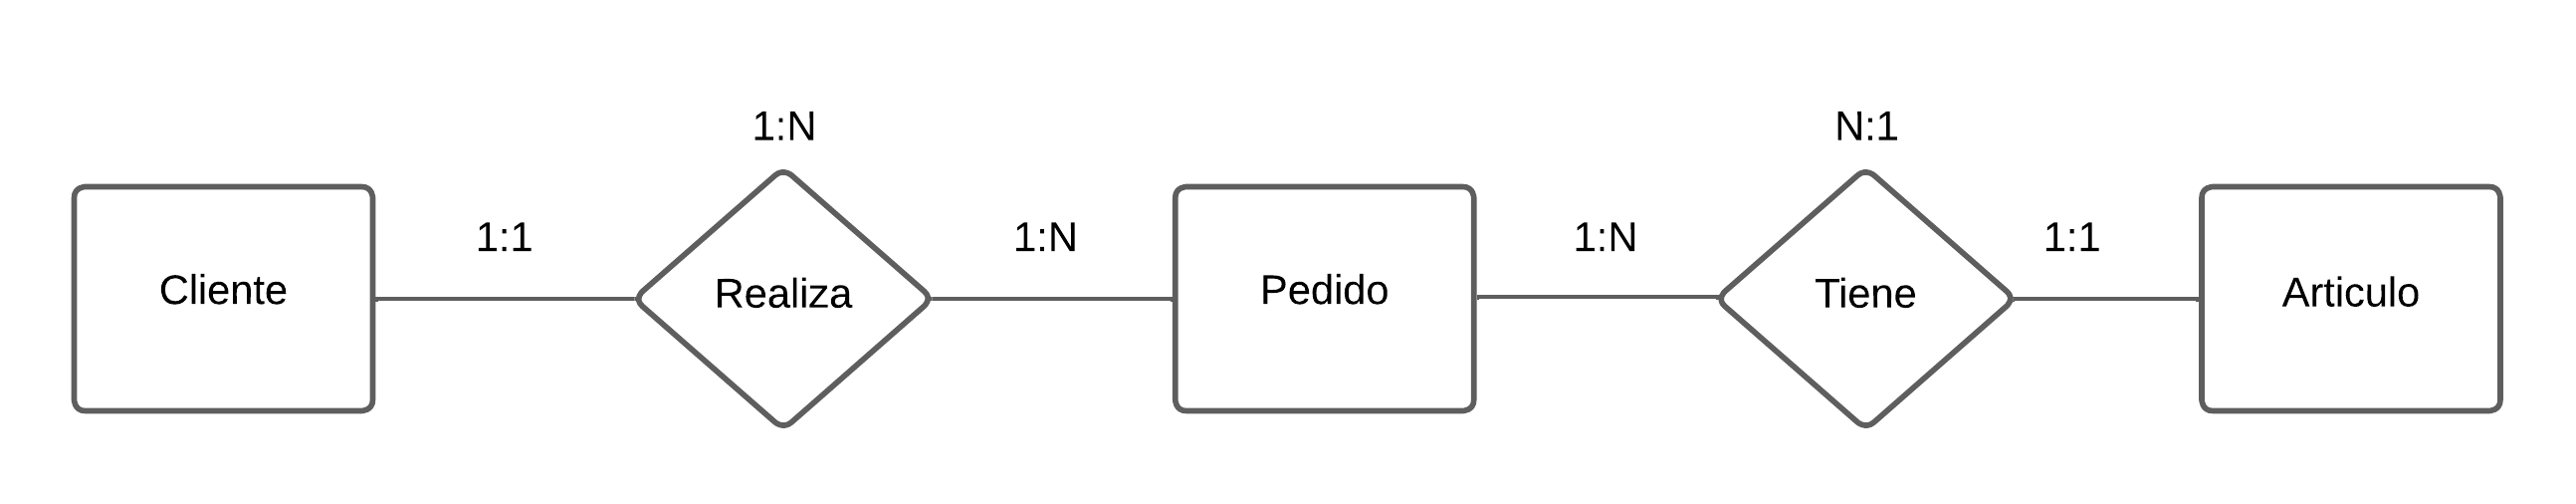
\includegraphics[width=\linewidth]{./Images/Punto_3.png}
	\end{center}
\end{figure}

\section{Diagrama E\@{}-\@{}R:\@{} Autos}

\begin{figure}[H]
	\begin{center}
		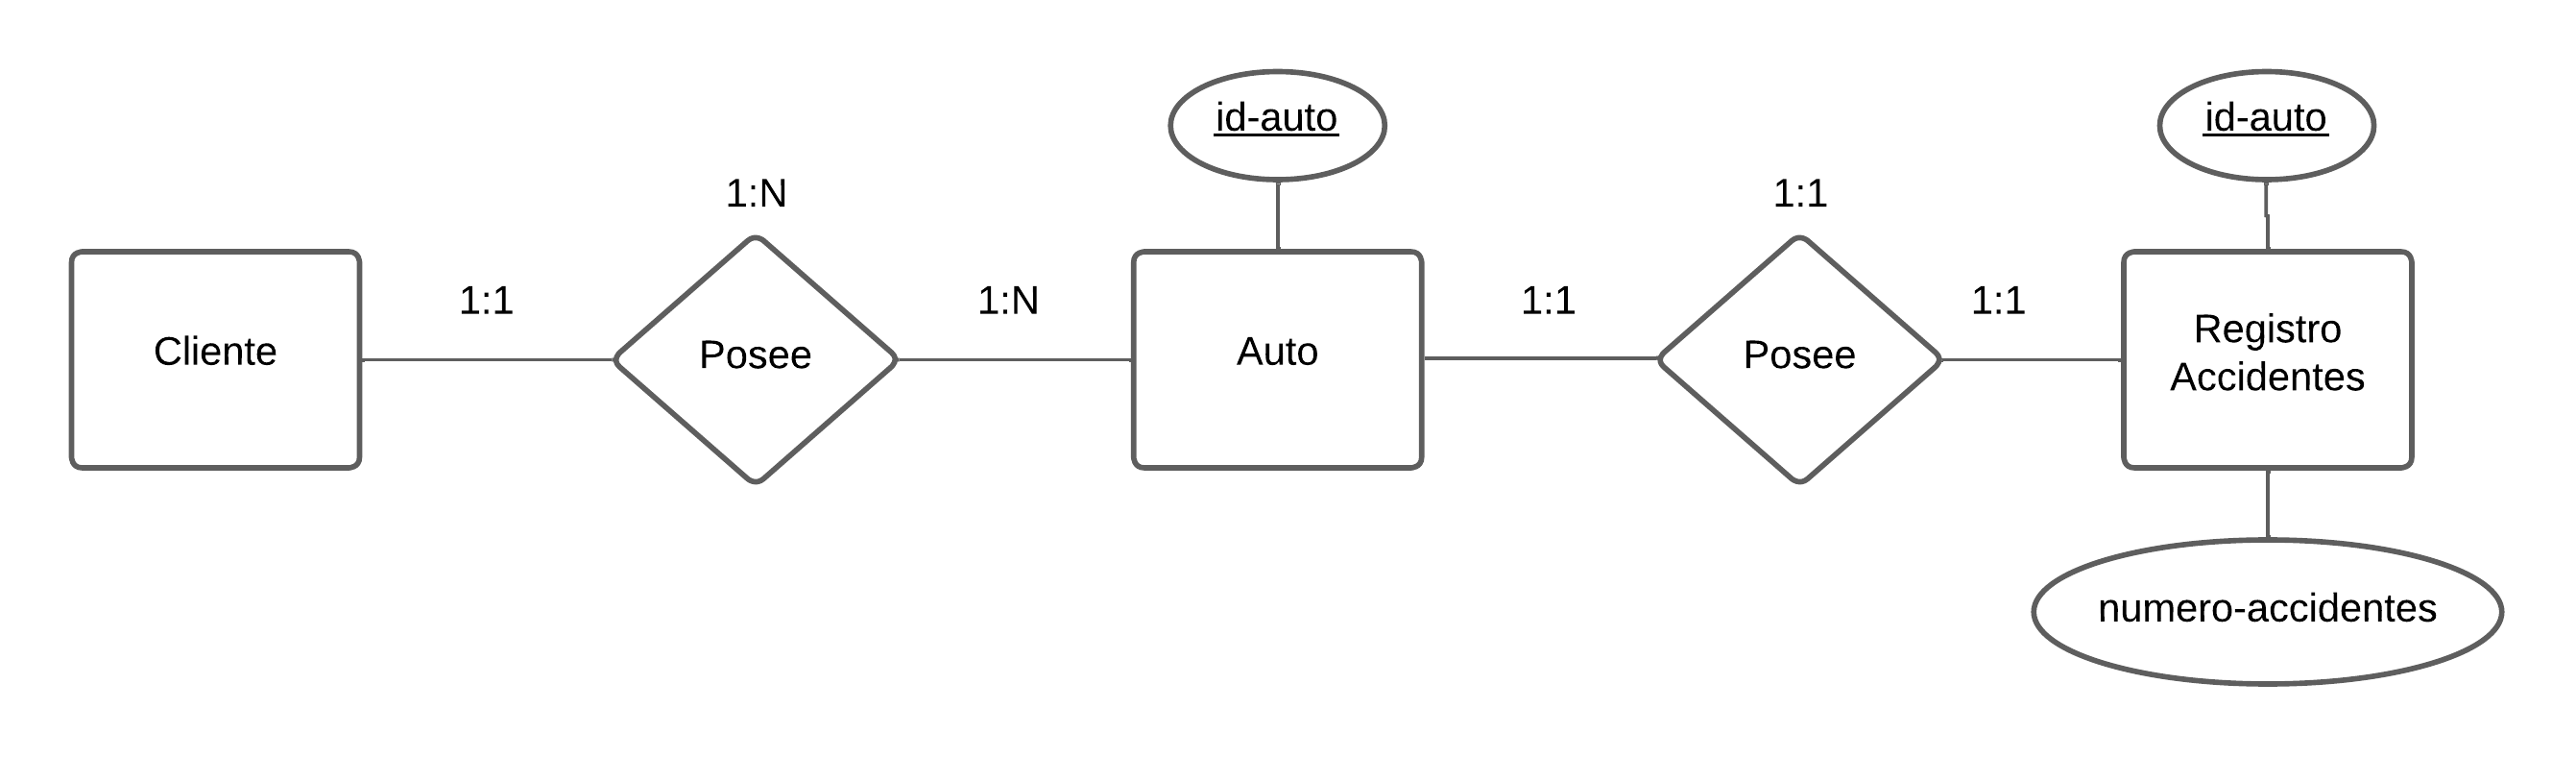
\includegraphics[width=\linewidth]{./Images/Punto_4.png}
	\end{center}
\end{figure}

\section{Diagrama E\@{}-\@{}R:\@{} Bookstore}

List the entity sets and their primary keys

\begin{itemize}[label=$\triangleright$]
	\item \bolditalic{Author}: Llave compuesta entre \textit{name} y \textit{address}
	\item \bolditalic{Publisher}: \textit{name}
	\item \bolditalic{Book}: \textit{ISBN}
	\item \bolditalic{Customer}: \textit{email}
	\item \bolditalic{Shopping-basket}: \textit{baskedID}
	\item \bolditalic{Warehouse}: \textit{code}
\end{itemize}

Suppose the bookstore adds Blu-ray discs and downloadable video to its
collection. The same item may be present in one or both formats, with
differing prices. Extend the E-R diagram to model this addition, ignoring
the effect on shopping baskets.

\begin{figure}[H]
	\begin{center}
		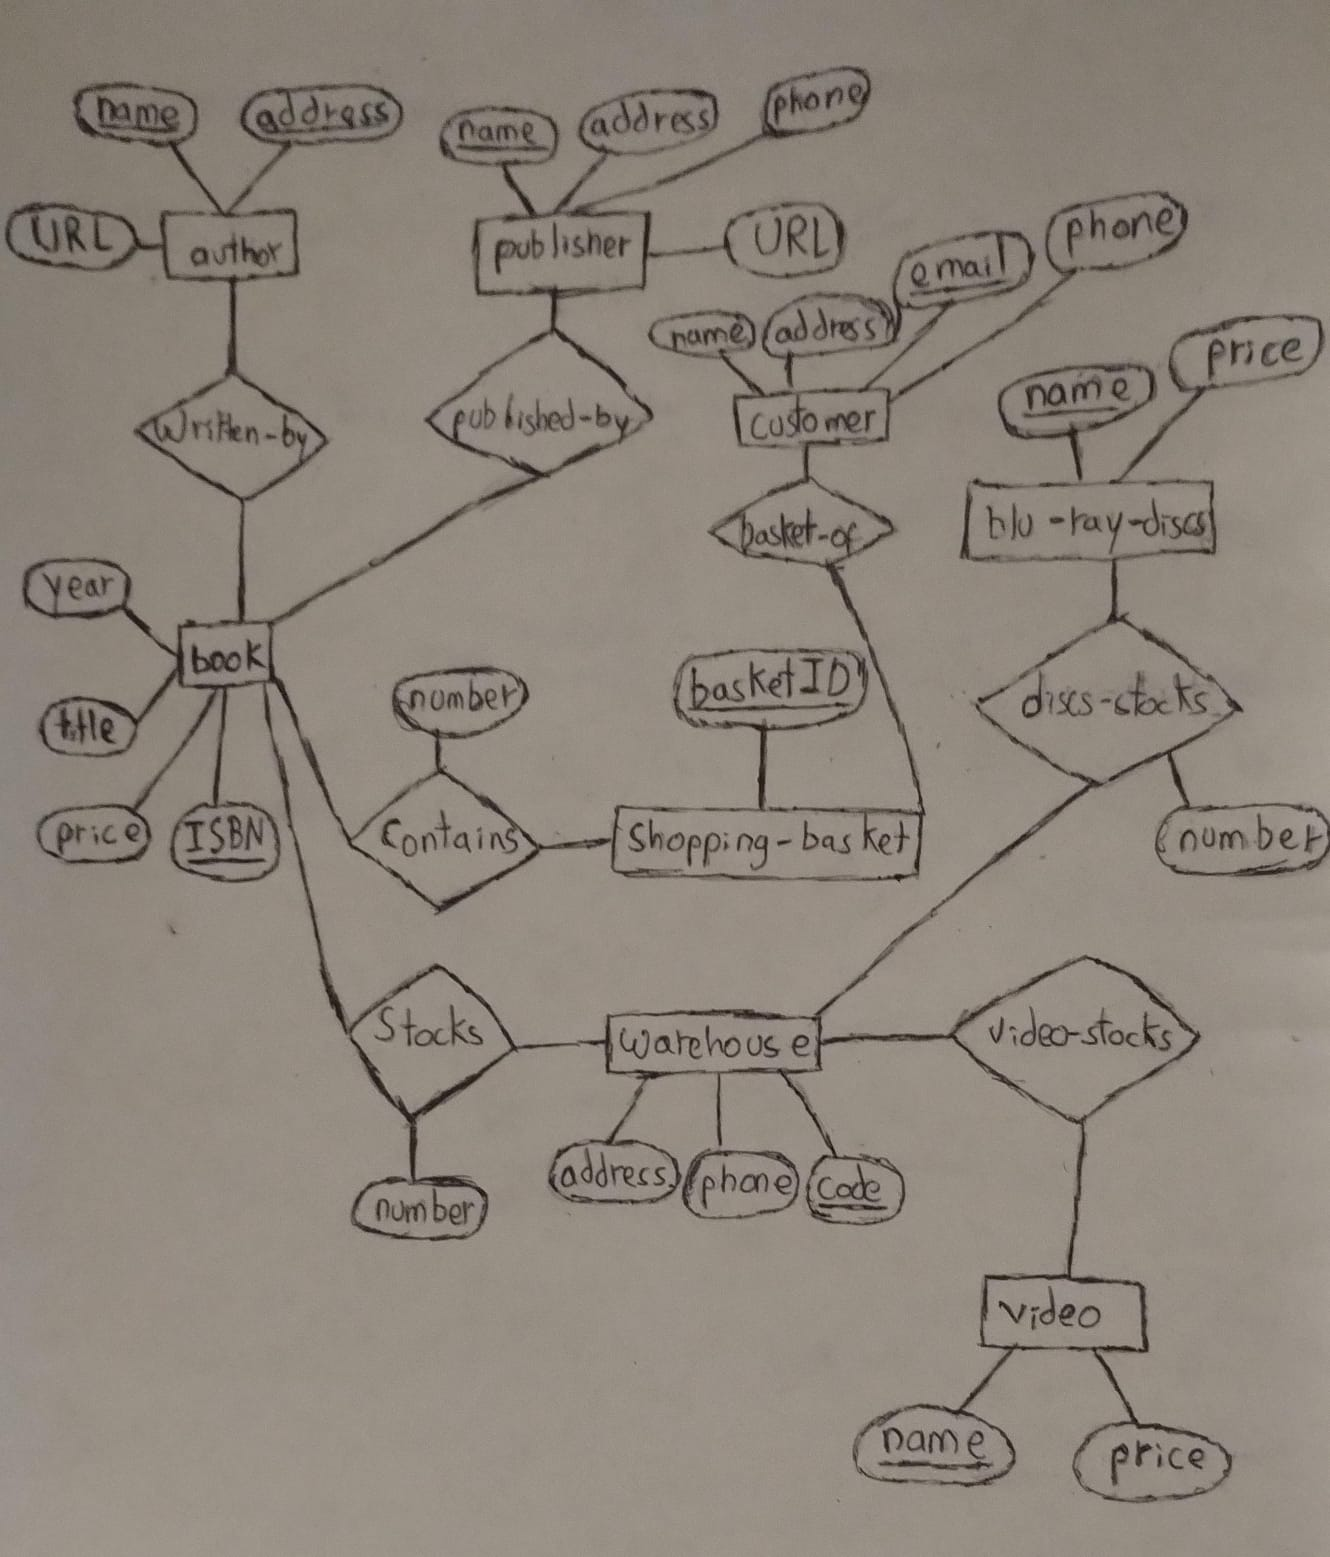
\includegraphics[width=\linewidth]{./Images/Punto_5b.jpeg}
	\end{center}
\end{figure}

\printbibliography

\end{document}